\documentclass[12pt]{article}
\usepackage[utf8]{inputenc}
\usepackage{amsmath,amssymb}
\usepackage{graphicx}
\usepackage{caption}
\usepackage{subcaption}

\usepackage[backend=bibtex]{biblatex}
\addbibresource{referencias.bib}

\title{Detecção de objetos }
\author{Fernando Pujaico Rivera}
\date{}

\begin{document}


\maketitle


%%%%%%%%%%%%%%%%%%%%%%%%%%%%%%%%%%%%%%%%%%%%%%%%%%%%%%%%%%%%%%%%%%%%%%%%%%%%%%%%
\section{Otimização dos parâmetros do sistema}
Como já foi visto em seções anteriores, para obter um ponto $P=(x,y,z)$ em 3D a partir de um ponto 
$p=(c_0,d_0,b_0)$ extraído a partir de imagens em 2D, é usada a função
$P \leftarrow func\_3d(p;\mathbf{K})$, sendo $\mathbf{K}=[h_0,D,\theta,f,g]^T$
um vetor que contem os parâmetros da geometria do sistema.
Porem, os valores em $\mathbf{K}\in \mathbb{R}^4$ inicialmente são medidos manualmente,
e precisam ser ajustados a sus valores reais, ou o mais próximos a estos que seja possível;
para cumprir este proposito podemos usar a função $func\_z()$ que é
uma simplificação da função $func\_3d()$ onde 
\begin{equation}
z \leftarrow func\_z(\{c_0,d_0\};\mathbf{K}),
\end{equation}
\begin{equation}
\hat{p}=\{c_0,d_0\}\quad \xrightarrow[\mathbf{K}]{func\_z} \quad z;
\end{equation}
de modo que o cálculo da altura $z$, mediante a função $func\_z()$,
só depende dos valores $\hat{p}=\{c_0,d_0\}$ e $\mathbf{K}$.
\begin{equation}\label{eq:setupz1}
func\_z(\hat{p};\mathbf{K})=\frac{
D~tg(\theta)
\left[
1+ ctg\left(\theta+atg\left(\frac{h_0}{d_0+c_0}\right)\right) ctg\left(\theta-atg\left(\frac{d_0}{h_0}\right)\right) 
\right]
}{
\left[1+ctg\left(\theta+atg\left(\frac{h_0}{d_0+c_0}\right)\right) ctg(\alpha)\right]
},
\end{equation}
\begin{equation}\label{eq:setupz2}
ctg(\alpha)=\frac{D~tg(\theta)ctg\left(\theta-atg\left(\frac{d_0}{h_0}\right)\right)- f}{g}.
\end{equation}
Usando todos estes antecedentes, nosso interesse é encontrar $\mathbf{K}$
com o valor mais ajustado a realidade; é dizer com valores optimizados,
com este fim são processados, e convertidas a imagens binarias, 
um conjunto de objetos de tamanho conhecido,
obtendo $L$ dados $\hat{p}_l$ e $z_l$, $\forall~1\leq l \leq L$.
Onde $z_l$ são as alturas dos objetos e $\hat{p}_l$ 
são os dados extraídos do objeto nas imagens binarias;
com a informação destes dois âmbitos (3D e 2D respetivamente)
definimos a função de custo $e\left(\mathbf{K}\right)$,
\begin{equation}\label{eq:setupz3}
e\left(\mathbf{K}\right)=\sum_{l=1}^{L} \left(z_l-func\_z(\hat{p}_l;\mathbf{K})\right)^2.
\end{equation}
Assim, se os valores $\mathbf{K}$, $\hat{p}_l$ e $z_l$, são medidos ou obtidos de forma exata,
$e\left(\mathbf{K}\right)$ deveria ser igual a zero, devido a que $z_l\approx func\_z(\hat{p}_l;\mathbf{K})$;
porem, como na prática usamos medidas e cálculos aproximados,
nosso objetivo mais eficiente é achar o vetor 
$\mathbf{K}=\mathbf{\bar{K}}$  que minimiza $e\left(\mathbf{K}\right)$.

Para facilitar o cálculo deste mínimo é conveniente expressar a Equação (\ref{eq:setupz3})
na forma matricial como na Equação (\ref{eq:setupz4})
\begin{equation}\label{eq:setupz4}
e\left(\mathbf{K}\right)=|| \mathbf{Z}-\mathbf{F}(\mathbf{K}) ||^2,
\end{equation}
onde $\mathbf{Z}\in \mathbb{R}^L$ é um vetor coluna, 
$\mathbf{F}(\mathbf{K}):\mathbb{R}^4 \rightarrow \mathbb{R}^L$ é uma 
função vetorial de variável vetorial $\mathbf{K}$, e o operador $||.||^2$ indica a norma ao quadrado do vetor,
\begin{equation}
\mathbf{Z}=
\begin{bmatrix}
z_1\\
z_2\\
\vdots\\
z_l\\
\vdots\\
z_L\\
\end{bmatrix},
\qquad
\mathbf{F}(\mathbf{K})=
\begin{bmatrix}
func\_z(\hat{p}_1;\mathbf{K})\\
func\_z(\hat{p}_2;\mathbf{K})\\
\vdots\\
func\_z(\hat{p}_l;\mathbf{K})\\
\vdots\\
func\_z(\hat{p}_L;\mathbf{K})\\
\end{bmatrix}.
\end{equation}
Assim, para minimizar a Equação (\ref{eq:setupz4}) podemos aplicar o
``algoritmo de Levenberg-Marquardt'' (LMA o simplesmente LM), 
tambem conhecido como o ``método de mínimos quadrados amortiguados'' (DLS)
\cite[pp. 232-234]{doicu2010numerical}.
De modo que o vetor $\mathbf{\bar{K}}$ que minimiza a  Equação (\ref{eq:setupz4})
é calculado iterativamente usando a  Equação (\ref{eq:setupz6}) 
\begin{equation}\label{eq:setupz6}
\mathbf{K}_{i+1}\leftarrow\mathbf{K}_{i}+ 
\left[\mathbf{J}(\mathbf{K}_i)^{T}\mathbf{J}(\mathbf{K}_i)+\alpha\mathbf{I}\right]^{-1}
\mathbf{J}(\mathbf{K}_i)^{T}\left[\mathbf{Z}-\mathbf{F}(\mathbf{K}_i)\right],
\end{equation}
onde $\mathbf{I}$ é uma matriz identidade de $4\times 4$, 
a variável $\alpha\geq 0$ é um fator de regularização escolhido por nos,
cujo propósito é conseguir que a matriz 
$\left[\mathbf{J}(\mathbf{K}_i)^{T}\mathbf{J}(\mathbf{K}_i)+\alpha\mathbf{I}\right]$
sempre tenha inversa, e 
 $\mathbf{J}(\mathbf{K})\in \mathbb{R}^{L\times 4}$ é a matriz jacobiana 
\cite[pp. 130]{zhang2017matrix} de $\mathbf{F}(\mathbf{K})$; é dizer
\begin{equation}
\mathbf{J}(\mathbf{K})=\frac{\partial \mathbf{F}(\mathbf{K})}{\partial \mathbf{K}^T}=
\begin{bmatrix}
\frac{\partial func\_z(\hat{p}_1;\mathbf{K})}{\partial \mathbf{K}^T}\\
\frac{\partial func\_z(\hat{p}_2;\mathbf{K})}{\partial \mathbf{K}^T}\\
\vdots\\
\frac{\partial func\_z(\hat{p}_L;\mathbf{K})}{\partial \mathbf{K}^T}\\
\end{bmatrix},
\end{equation}
\begin{equation}\label{eq:setupz9}
\frac{\partial func\_z(\hat{p};\mathbf{K})}{\partial \mathbf{K}^T}\equiv 
\begin{bmatrix}
\frac{\partial func\_z(\hat{p};\mathbf{K})}{\partial h_0} &
\frac{\partial func\_z(\hat{p};\mathbf{K})}{\partial D} &
\frac{\partial func\_z(\hat{p};\mathbf{K})}{\partial \theta} &
\frac{\partial func\_z(\hat{p};\mathbf{K})}{\partial f} &
\frac{\partial func\_z(\hat{p};\mathbf{K})}{\partial g}
\end{bmatrix}.
\end{equation}
Finalmente a Equação (\ref{eq:setupz6}) converge a um vetor $\mathbf{K}_{i+1}$ que é um mínimo global 
de $e\left(\mathbf{K}\right)$, se inciamos o cálculo iterativo desde 
um valor $\mathbf{K}_0$ próximo à solução, neste caso são usados os valores
$\{h_0,D,\theta,f,g\}$ medidos o calculados manualmente. 
As iterações finalizam quando $\mathbf{K}_{i+1}\approx \mathbf{K}_{i}$
onde se declara que o valor ótimo $\mathbf{\bar{K}}\equiv \mathbf{K}_{i+1}$.

Sobre o cálculo das derivadas parciais da função
$func\_z(\hat{p};\mathbf{K})$ em relação a $\mathbf{K}$, como
descrito na Equação (\ref{eq:setupz9}), é fácil observar que estes cálculos
são possíveis porem extremadamente laboriosos;
por este motivo foi usado o motor de cálculo simbólico  
e  sistema de álgebra computacional: Maxima \cite{santos2009introduccao}.
Assim, com a ajuda desse software é calculado de forma simbólica
as derivadas parciais da função $func\_z(\hat{p};\mathbf{K})$ em relação a $\mathbf{K}$.

Todo o processo de optimização antes descrito pode ser sistematizado mediante o diagrama de blocos 
da Figura \ref{fig:Diagrama6}, onde podemos ver 3 entradas de dados e uma saída,
que neste caso é o valor de $\mathbf{K}=\mathbf{\bar{K}}$ que minimiza $e\left(\mathbf{K}\right)$.
\begin{figure}[!h]
     \centering
         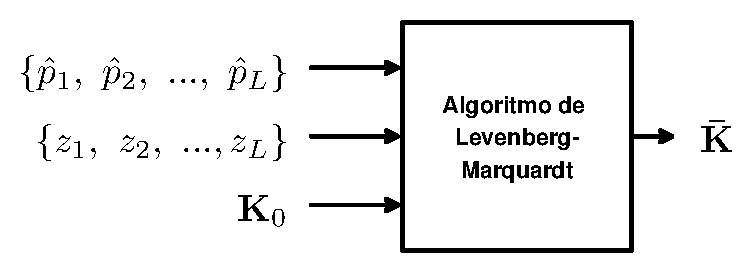
\includegraphics[width=0.7\textwidth]{Diagrama6.eps}
\caption{Algoritmo de Levenberg-Marquardt.}
\label{fig:Diagrama6}
\end{figure}
\printbibliography
\end{document}
